%%%%%%%%%%%%%%%%%%%%%%%%%%%%%%%%%%%%%%%%%%%%%%%%%%%%%%%%%%%%%%%
% P3b MLP
% David Miguel Lozano
% Javier Martínez Riberas
% Universidad de Burgos - Noviembre 2016
%%%%%%%%%%%%%%%%%%%%%%%%%%%%%%%%%%%%%%%%%%%%%%%%%%%%%%%%%%%%%%%

% -------------------------------------------------------------
% Preamble
% -------------------------------------------------------------
\documentclass[a4paper,12pt,titlepage]{article}

% -------------------------------------------------------------
% Packages
% -------------------------------------------------------------
\usepackage[utf8]{inputenc}	% Unicode support
\usepackage[T1]{fontenc}		% Font encoding
\usepackage[spanish]{babel}	% Languaje
\usepackage{lmodern}	% Typeface 
\usepackage{textcomp} % Special symbols
\usepackage{graphicx}	% Add pictures
\usepackage{pgfplots} % Graphs and charts
\usepackage{hyperref}	% Add a link to index entries
\usepackage{amsmath}	% Advanced math typesetting
\usepackage{amsfonts}	% Mathematical formulas
\usepackage{amssymb}	% Extended symbol collection
\usepackage{listings}	% Code formatting and highlighting
\usepackage{algorithm}   % Psudocódigos
\usepackage{algorithmic} % Psudocódigos
\usepackage{xcolor}		% Color package
\usepackage{enumitem}	% Customizing lists
\usepackage{parskip}	% Paragraph styles
\usepackage[a4paper]{geometry} 		% Margins
\usepackage[numbers,sort]{natbib}	% Bibliography management
\usepackage{booktabs}							% Tables

% -------------------------------------------------------------
% Configuration
% -------------------------------------------------------------
% Images path
\graphicspath{ {img/} }
% Graphs configuration 
\pgfplotsset{width=\textwidth,compat=1.9}
% Hyperlinks coloring
\hypersetup{
	colorlinks,
	linkcolor={green!40!black},
	citecolor={blue!50!black},
	urlcolor={blue!80!black}
}
% Define HRule
\newcommand{\HRule}[1]{\rule{\linewidth}{#1}}
% Define listings styles
\definecolor{codebg}{HTML}{EEEEEE}
\definecolor{codeframe}{HTML}{CCCCCC}
\definecolor{comments}{HTML}{009900}
\lstset{
  language=Matlab, 								% Programming language 
  backgroundcolor=\color{codebg},	% Background color
  frame=single, 									% Add frame around code
	framesep=10pt,									% Padding
	rulecolor=\color{codeframe},		% Don't change frame color
	upquote=true,										%
	breakatwhitespace=true,					% Break line only in spaces
	keepspaces=true,								% Keep indentation
	tabsize=2,											% Tab size
	title=\lstname, 								% Show filename as caption
	basicstyle=\ttfamily, 					% Size and font
  keywordstyle=\color{black}\ttfamily,
	commentstyle=\color{comments},	% Color of comments
  morecomment=[l][\color{magenta}]{\#}
}
% Define style table
\setlength{\heavyrulewidth}{1.5pt}
\setlength{\abovetopsep}{4pt}
\begin{document}
% -------------------------------------------------------------
% Cover
% -------------------------------------------------------------
\author{David Miguel Lozano \ Javier Martínez Riberas}
\title{Optimización por Enjambre (Particle Swarm Optimization)}
\date{07-11-2016}

\begin{titlepage}
	\centering
	
\includegraphics[width=0.16\textwidth]{ubu-logo.png}\par
	\vspace{0.3cm}
	{\scshape\LARGE Universidad de Burgos \par}
	\vfill
	{\scshape\Large Computación Neuronal y Evolutiva \par}
	\HRule{2pt}
	{\huge\bfseries Optimización por Enjambre (\textit{Particle Swarm Optimization}) \par}
	\HRule{2pt}
	\\ [0.5cm]
	{La optimización por enjambre de partículas (\textit{Particle Swarm Optimization} - PSO) hace referencia a una metaheurística que evoca el comportamiento de algunos animales como enjambres de insectos en la naturaleza.}
	\vfill
	Estudiantes:\par
	{\Large\scshape David Miguel Lozano \\ Javier Martínez Riberas \par}
	\vfill
	Profesores de la asignatura:\par
	\textsc{Álvaro Herrero Cosío \\ Bruno Baruque Zanón}
	\vfill
	{\large 1º semestre 2016 \par}
\end{titlepage}

% -------------------------------------------------------------
% Contents
% -------------------------------------------------------------
\newpage
\tableofcontents
\begin{appendix}
  %\listoffigures
  %\listoftables
\end{appendix}

% -------------------------------------------------------------
% Body
% -------------------------------------------------------------
\newpage

\section{Introducción}

La optimización por enjambre de partículas (\textit{Particle Swarm Optimization} - PSO) es un algoritmo metaheurístico que hace una búsqueda iterativa en el espacio de soluciones posibles para intentar mejorar las soluciones actuales.

Fue desarrollado por James Kennedy y Russell Eberhart en 1995, partiendo de una simulación simplificada de un entorno social basado en una parvada.

La principal inspiración del PSO es la vida artificial (\textit{A-life}) en general, con el estudio de bandadas de aves, bancos de peces o la inteligencia de enjambre en particular. Aunque, según mencionan los autores en su trabajo original \citep{Kennedy1995}, también se inspira en campos como los algoritmos genéticos y la computación evolutiva.

Sus aplicaciones principales son problemas no lineales y multidimensionales, aunque se puede adaptar a casi todo tipo de problemas.

\section{Historia}

En 1995, James Kennedy y Russell Eberhart publicaron el artículo “\textit{Particle Swarm Optimization}”\citep{Kennedy1995}, en el que propusieron una prueba de concepto para optimizar funciones no lineales basándose en la metodología de enjambre de partículas. 

El objetivo inicial de los autores era realizar una simulación gráfica de un modelo de conducta social basado en el movimiento imprevisible de una bandada de aves. Sin embargo, posteriormente descubrieron que su modelo podía ser utilizado como un optimizador.

En su primera aproximación, la velocidad de cada agente (en su caso pájaros) se ajustaba en relación con la velocidad de su vecino más próximo. Sin embargo, este método desembocaba en que la parvada establecía rápidamente una dirección fija.

Para solventar este problema, introdujeron una variable estocástica llamada “locura”. De tal manera, que en cada iteración se añadía algún cambio aleatorio. Lo que proporcionaba un aspecto más real a la simulación, aunque la variación seguía siendo totalmente artificial.

Inspirados por la simulación de aves de Hepner, se propusieron añadir un objetivo a los agentes: encontrar comida. Para esto, modificaron los agentes para que cada uno supiese en todo momento la mejor posición global de cada uno y cambiaron el ajuste de las velocidades de acuerdo a estos valores.

Por lo tanto, el escenario planteado era el siguiente: una bandada de pájaros se encuentra buscando comida aleatoriamente en un área donde sólo hay una pieza de comida. Ninguno de los pájaros sabe donde está la comida, pero, debido a la función a optimizar elegida, sí que saben cómo de lejos están de ella.

Con las modificaciones introducidas, vieron como las aves eran capaces de encontrar la comida gracias a la forma en la que el conocimiento de cada individuo era compartida en el medio social. Los resultados eran muy buenos, estas se aproximaban a la comida de forma realística y sincronizada, hasta que finalmente se “posaban” en el objetivo. De esta forma, demostraron que el método era capaz de optimizar funciones lineales de dos dimensiones.

En una nueva aproximación, se intentó generalizar el método a un entorno no lineal y multidimensional. Para ello, se utilizó una matriz de vectores para guardar las velocidades de cada dimensión. Se probó la nueva versión con diferentes problemas, entre ellos, el entrenamiento de varias redes neuronales. Para todos ellos, el algoritmo arrojó unos buenos resultados.

El algoritmo resultante, tras algunas mejoras y optimizaciones posteriores, sentó las bases de la optimización por enjambre de partículas.

El término enjambre había sido definido por Millonas en 1993 en el artículo “\textit{Swarms, phase transitions, and collective intelligence}”\citep{millonas_swarms_1993}. En él, se establecen los cinco principios que deben cumplir los enjambres inteligentes: 

\begin{enumerate}[noitemsep]
	\item \textbf{Principio de proximidad:} la población tiene que ser capaz de realizar cálculos simples del espacio y tiempo.
	\item \textbf{Principio de calidad:} la población tiene que ser capaz de responder a factores de calidad en el entorno.
	\item \textbf{Respuestas diversas:} la población no debe llevar a cabo sus acciones por canales excesivamente estrechos.
	\item \textbf{Estabilidad:} la población no debe de cambiar su modo de comportamiento cada vez que cambia el entorno.
	\item \textbf{Adaptabilidad:} la población tiene que poder cambiar su modo de comportamiento cuando merezca la pena computacionalmente.
\end{enumerate}

El término partículas fue escogido por compromiso. Al tratarse de agentes sin masa ni volumen podían haberse denominado puntos. Sin embargo, se quiso incidir en las propiedades de velocidad y aceleración que estos poseen. Por esto, se vio más adecuado el uso del término partículas. \citep{Kennedy1995}

En una nueva publicación en 1998 \citep{Shi1998}, Shi y Eberhart discutieron la necesidad de utilizar la velocidad en la propia ecuación de actualización de la velocidad. Si se eliminaba, PSO dejaba de explorar y se limitaba a explotar los mínimos locales. Si no se eliminaba, PSO gastaba demasiado tiempo en explorar, en vez de intentar buscar el mínimo local que podría ser el global.

Para poder generalizar un comportamiento intermedio entre búsqueda exploratoria y explotación local, propusieron añadir una variable nueva. Esta variable multiplica la velocidad, de manera que, cuando es mayor de 1 fomenta la exploración y cuando es menor fomenta la explotación.

En la solución propuesta, la variable se inicializa por encima de 1 y se va decrementando linealmente hasta llegar a 0 en el número máximo de iteraciones. De esta manera, el algoritmo prioriza la exploración en una etapa inicial, pero se centra en la explotación según avanza la ejecución.

En la actualidad se están desarrollando nuevas y más sofisticadas variantes del PSO con el fin de mejorar el rendimiento de este. En particular, se está trabajando en las siguientes vías de investigación: \citep{Zhang2015}

\begin{itemize}[noitemsep]
	\item Modificaciones del PSO (quantum-behaved PSO, bare-bones PSO, chaotic PSO, fuzzy PSO, PSOT-VAC, opposition-based PSO, etc.).
	\item Métodos híbridos que combinan PSO con otros métodos metaheurísticos, incluyendo algoritmos genéticos (GA), sistemas inmunológicos artificiales (AIS), búsqueda Tabú (TB), algoritmos de colonias de hormigas (ACO), algoritmos de recocido simulado (SA), algoritmos de colonias de abejas artificiales (ABC), evolución diferencial (DE), optimizaciones biogeográficas (BBO), búsquedas armónicas (HS), etc.
	\item Extensión del PSO a otros campos de optimización, como optimización multiobjetivo, con restricciones, discreta o binaria.
	\item Análisis teóricos del PSO. Sobretodo en la selección de parámetros y análisis de convergencia.
	\item Implementaciones paralelas de PSO: incluyendo programación multinúcleo, en GPU o en Cloud.
\end{itemize}

\section{Funcionamiento}

El funcionamiento es muy simple. Sin embargo, aunque hay varias teorías acerca de porqué funciona, los expertos no consiguen ponerse de acuerdo en una.

En PSO, las potenciales soluciones se llaman partículas y “vuelan” por el espacio del problema siguiendo a las partículas óptimas actuales. 

Cada partícula posee unas coordenadas en el espacio del problema. Estas están asociadas con la mejor solución (\textit{fitness}) encontrada hasta ahora. A su vez, cada partícula almacena tres valores:

\begin{itemize}[noitemsep]
	\item velocidad: dirige el “vuelo” de la partícula.
	\item \lstinline|pbest|: el valor de la mejor solución que ha encontrado hasta el momento (\textit{fitness}).
	\item \lstinline|gbest|: el valor de la mejor solución encontrada hasta el momento por cualquier partícula del enjambre.
\end{itemize}

El algoritmo se inicializa con un grupo de partículas aleatorias (soluciones) y posteriormente busca la solución óptima mediante la actualización de estas.

En cada iteración, se actualiza la velocidad de cada partícula siguiendo sus dos “mejores” valores: \lstinline|pbest| y  \lstinline|gbest|. Y con su velocidad se calcula su nueva posición.

En concreto, se actualiza la velocidad de cada dimensión de acuerdo a la siguiente expresión:

\begin{lstlisting}
vx[][]= vx[][] +
		2 * rand() * (pbestx[][] - presentx[][]) +
		2 * rand() * (pbestx[][gbest] - presentx[][])
\end{lstlisting}

Esta expresión actualiza la velocidad de una dimensión (\lstinline|vx[][]|) de tal manera que la partícula se acerque al mejor punto conocido por esta. \lstinline|presentx| hace referencia a la partícula actual (solución), \lstinline|rand()| genera un número aleatorio entre (0, 1), \lstinline|pbestx| y \lstinline|pbestx| se corresponden con los valores descritos anteriormente.

La posición se actualiza de acuerdo a:

\begin{lstlisting}
presentx[][]=presentx[][]+vx[][]
\end{lstlisting}

El pseudocódigo del algoritmo es el siguiente:
\newpage

\begin{algorithm}[!ht]
	\begin{algorithmic}[1]
	\FORALL{partículas} 
		\STATE Inicializar partícula con un vector aleatorio uniformemente distribuido.
		\STATE Inicializar pbest con su posición inicial.
		\IF{fitness en pbest es mejor que en gbest}
			\STATE Actualizar gbest con pbest.
		\ENDIF
		\STATE Inicializar velocidad de la partícula.
	\ENDFOR
	\REPEAT 
		\FORALL{partículas} 
			\STATE Calcular el valor de fitness.
			\IF{fitness actual es mejor que en gbest}
				\STATE Actualizar gbest con la posición actual.
			\ENDIF
		\ENDFOR
		\STATE Obtener la partícula con el mejor fitness.
		\FORALL{partículas} 
			\STATE Calcular su nuevo valor de velocidad.
			\STATE Actualizar su posición.
		\ENDFOR		
	\UNTIL{no se cumpla el criterio de parada (iteraciones máx./error mín.)}
	\STATE Devolver gbest como solución encontrada.
	\end{algorithmic}
\caption{PSO básico.}
\label{alg:algoritmoRaro}
\end{algorithm}

En las siguientes figuras podemos observar dos instantes consecutivos del algoritmo. El sentido de la velocidad de cada partícula está indicada con una flecha. Vemos como el mejor resultado obtenido en el primer instante condiciona el movimiento de las partículas en el segundo.

Para visualizar gráficamente el funcionamiento del algoritmo se han grabado dos simulaciones realizadas en Matlab:

\begin{itemize}[noitemsep]
	\item Simulación 2D: [\href{https://raw.githubusercontent.com/davidmigloz/evolutionary-computation/master/T1_PSO/res/pso_demo_2d.webm}{webm}][\href{https://raw.githubusercontent.com/davidmigloz/evolutionary-computation/master/T1_PSO/res/pso_demo_2d.flv}{flv}]
	\item Simulación 3D: [\href{https://raw.githubusercontent.com/davidmigloz/evolutionary-computation/master/T1_PSO/res/pso_demo_3d.webm}{webm}][\href{https://raw.githubusercontent.com/davidmigloz/evolutionary-computation/master/T1_PSO/res/pso_demo_3d.flv}{flv}]
\end{itemize}

\newpage

\begin{figure}[!ht]
\centering
\begin{minipage}{.5\textwidth}
  \centering
  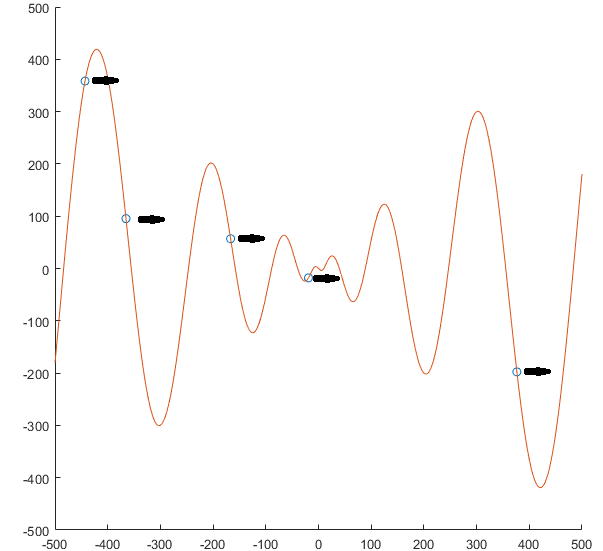
\includegraphics[width=\textwidth]{1.png}
  \caption{PSO t0}
  \label{fig:1}
\end{minipage}%
\begin{minipage}{.5\textwidth}
  \centering
  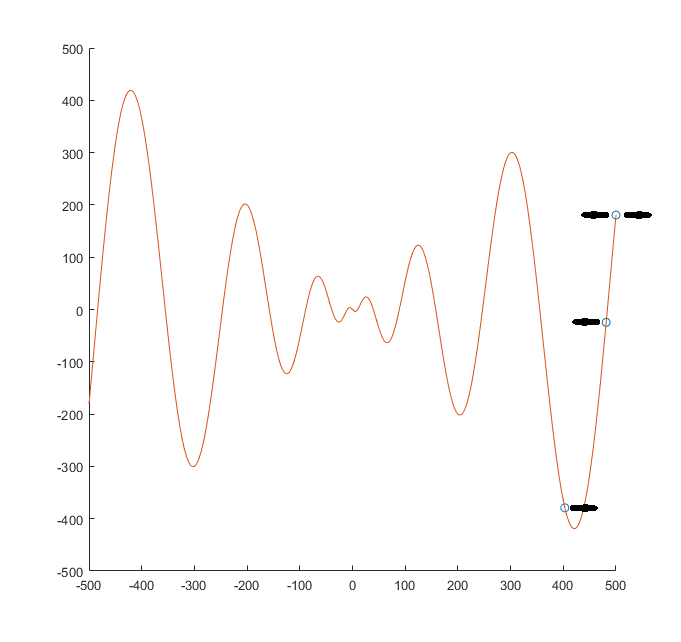
\includegraphics[width=\textwidth]{2.png}
  \caption{PSO t1}
  \label{fig:2}
\end{minipage}
\end{figure}

El número de parámetros a ajustar en PSO no es muy grande: \citep{xiaohui_hu_particle}

\begin{itemize}[noitemsep]
	\item \textbf{Número de partículas:} el rango típico está entre 10 y 40 partículas. Para la mayoría de problemas 10 partículas es un número suficiente para obtener buenos resultados. Sin embargo, en problemas difíciles el número necesario se puede incrementar hasta las 100 o 200 partículas.
	\item \textbf{Dimensiones:} determinado por el problema a resolver.
	\item \textbf{Rangos:} los valores por lo que puede moverse cada partícula. También es particular del problema a resolver. Los rangos pueden ser diferentes en cada dimensión.
	\item \textbf{Velocidad máxima:} define el máximo cambio que puede sufrir una partícula en una iteración. Normalmente se establece con el valor del rango.
	\item \textbf{Condición de parada:} se suele utilizar un criterio doble. Por un lado se define el número máximo de iteraciones y por otro una cota inferior del error. Estos valores dependen del problema a resolver.
\end{itemize}

El por qué PSO funciona no está claro, como ya hemos comentado anteriormente. Existen dos teorías principales sobre su funcionamiento interno. \citep{_particle_2016}

La primera teoría y más extendida defiende que PSO realiza dos tipos de búsqueda. En un primer momento, realiza una búsqueda exploratoria amplia en el espacio de soluciones (comportamiento de exploración). Pero según aumenta el tiempo, cambia a una búsqueda local que se aproxima rápidamente hacia un óptimo, posiblemente local (comportamiento de explotación).

La otra teoría defiende que aún no se ha logrado comprender cómo afecta el comportamiento del enjambre a la calidad del proceso de optimización, especialmente en problemas de optimización con espacios de búsqueda multidimensionales, discontinuos o variables en el tiempo. Esta escuela de pensamiento no busca un equilibrio entre las fases de exploración y explotación, sino que busca encontrar los mejores parámetros posibles para el problema en concreto. Este planteamiento ha llevado a simplificar los algoritmos de PSO en variantes como \textit{Bare Bones PSO} \citep{Kennedy2003} o la optimización con enjambre de partículas aceleradas (\textit{Acelerated PSO} - APSO). Ambos métodos prescinden de la velocidad.

\section{Aplicaciones}

Desde que se desarrolló el método de optimización por enjambre de partículas, se ha aplicado en numerosos campos. 

Al tratarse de una metaheurística, tiene un carácter muy generalista para resolver cualquier problema que se pueda definir en términos de un problema de optimización. Aunque, como cualquier otra metaheurística, no asegura encontrar una solución óptima. 

Una de las ventajas de PSO frente a otras metaheurísticas es que no usa descenso de gradiente. Por lo tanto, no es necesario que la función que define el problema sea derivable.

Otra de sus características positivas es el reducido número de parámetros que hay que ajustar. La misma versión del algoritmo con muy ligeras modificaciones puede resolver problemas muy diferentes.

Además, ha demostrado obtener buenos resultados de una manera más rápida y barata que muchos otros métodos de optimización.

Por todo lo anterior, PSO ha sido utilizado en infinidad de aplicaciones. A continuación exponemos las más relevantes clasificadas por categorías por orden de popularidad: \citep{Poli2008,Zhang2015}

\subsection{Data mining}

Un buen número de aplicaciones están relacionadas con tareas de agrupamiento, clasificación, reducción de la dimensionalidad o selección de características. Que a su vez, pueden ser utilizadas para tareas de predicción como el pronóstico del tiempo, la carga de la red eléctrica, tráfico de vehículos, etc.

\subsection{Inteligencia artificial}

El uso principal de PSO en cuanto a la inteligencia artificial son las redes neuronales, tanto su control y diseño, como el entrenamiento. Fue la primera aplicación propuesta por los autores del PSO. También, se han desarrollado algorítmos híbridos que combinan genéticos y PSO.

\subsection{Medicina}

Otro campo popular es la biomedicina. En donde se utiliza en aplicaciones muy diversas, desde herramientas para el diagnóstico de Parkinson, diseño de medicamentos, prótesis, clasificación de cánceres, agrupamiento de genes, selección de biomarcadores, etc.

\subsection{Operaciones}

Los PSO son ampliamente utilizados en tareas de control y planificación . Como planificaciones óptimas de procesos, calendarios laborales, horarios de trenes, redes eléctricas, etc.

\subsection{Telecomunicaciones}

El campo más popular del PSO son las telecomunicaciones. Su uso por excelencia es el diseño de antenas de telecomunicaciones, de tal forma que optimicen la propagación o la recepción de la señal. Otros usos en este campo son el diseño y optimización de todo tipo de redes de comunicaciones. Por ejemplo, la elección del emplazamiento óptimo de los equipos, la optimización del ancho de banda y la asignación de canales, redes inalámbricas, etc.

\subsection{Procesamiento de imagen y sonido}

Este es uno de los campos donde PSO tiene una gran repercusión. Existen infinidad de aplicaciones desde reconocimiento de caras, iris, peatones, frutas, detección de defectos, clasificación de objetos, reducción de ruido, tracking de objetos, filtros adaptativos, codificación de sonido, gráficos 3D, síntesis de texturas, etc.

\subsection{Robótica}

En el campo de la ingeniería eléctrica, electrónica y de automatismos también existe un importante número de artículos relacionados con PSO. Desde diseño digital de circuitos electrónicos tolerantes a fallos, planificación de trayectos, hasta el control y planificación de motores.




\section{Comparación}

PSO comparte ciertas similitudes con técnicas de computación evolutiva como los algoritmos genéticos:

\begin{itemize}[noitemsep]
	\item El sistema es inicializado con una población de soluciones aleatorias.
	\item El valor de fitness de cada individuo se recalcula en cada iteración.
	\item El sistema busca la solución óptima mediante la actualización de sus generaciones.
	\item Ambos introducen valores aleatorios en su búsqueda del óptimo.
	\item Ninguno de los dos métodos garantiza encontrar la solución óptima.
	\item Ambos pueden resolver cualquier problema que se pueda formular como un problema de optimización.
\end{itemize}

Pero también poseen notables diferencias:

\begin{itemize}[noitemsep]
	\item En la actualización de generaciones, PSO no utiliza operadores evolutivos como la selección, el cruce o la mutación, sino que sus nuevos individuos se basan en los individuos óptimos actuales.
	\item Cada partícula posee memoria. Lo que supone una pieza clave del algoritmo.
	\item El mecanismo por el que se comparte información es diferente. En PSO, se utiliza un mecanismo de comunicación unidireccional mediante el cual sólo se comparte el valor  \lstinline|gbest| entre partículas.
	\item La velocidad de convergencia suele ser mayor que la de los algoritmos genéticos.
	\item Poseen menos parámetros configurables.
\end{itemize}

Uno de los usos que se les da a los algoritmos genéticos es para el entrenamiento de redes neuronales. Los pesos y/o la topología de la red se codifican como genotipos y se diseña una función de selección de acuerdo con los objetivos de la red. Por ejemplo, para un problema de clasificación, el valor de fitness puede ser el ratio de patrones clasificados mal.

Sin embargo, hay varios artículos que proponen el uso de PSO para reemplazar el algoritmo de entrenamiento \textit{back-propagation}. Ya que es un método rápido y obtiene buenos resultados en la mayoría de los casos. Además, posee ciertas ventajas respecto a los algoritmos genéticos, en los que la selección de los operadores genéticos debe realizarse cuidadosamente.

\section{Conclusiones}

En este trabajo se ha introducido el método de optimización por enjambre de partículas. Como se ha visto, se trata de un algoritmo simple que permite optimizar un amplio abanico de funciones.

Como todos los métodos de optimización, PSO posee una serie de ventajas e inconvenientes. Es un algoritmo simple, con un número reducido de parámetros, puede optimizar funciones no derivables y es eficiente en un gran número de casos. Por otro lado, en su versión original, puede quedarse atrapado en mínimos locales, su complejidad computacional es algo elevada y su rendimiento es muy sensible a la parametrización escogida.

PSO ha sido utilizado en numerosas aplicaciones pertenecientes a disciplinas científicas muy diferentes. Desde su primera aplicación para en entrenamiento de redes neuronales, hasta la síntesis de medicamentos en medicina, optimización de las redes de comunicaciones y eléctricas, planificación de calendarios laborales o métodos de visión artificial.

Desde su aparición, la investigación del PSO creció de forma exponencial hasta el año 2009, llegando a publicarse más de 2.000 artículos en un año. Actualmente, la investigación se ha estabilizado, pero sigue habiendo un gran interés en la materia.

Teniendo en cuenta lo anterior, podemos afirmar que PSO está todavía en una fase joven y que le queda bastante camino por recorrer. Como hemos visto, existen varias líneas de investigación a día de hoy, y varias de ellas parecen prometedoras. El tiempo dirá si PSO consigue establecerse como algoritmo de referencia en algún campo en concreto.
	
\begin{tikzpicture}
\begin{axis}[
	xticklabel style = {font=\tiny},
	x tick label style={
		/pgf/number format/1000 sep=},
	xlabel={Año},
	ylabel={Artículos sobre PSO},
	ybar=1pt,
	bar width=9pt,
	enlargelimits=0,
	ybar interval=0.7,
]
\addplot 
	coordinates {(1995, 5)(1996, 0)(1997, 3)(1998, 7)(1999, 11)(2000, 13)(2001, 18)(2002, 78)(2003, 109)(2004, 240)(2005, 350)(2006, 676)(2007, 886)(2008, 1382)(2009, 1945)(2010, 2174)(2011, 1674)(2012, 1677)(2013, 1557)(2014, 1674)(2015, 1729)(2016, 0)};
\end{axis}
\end{tikzpicture}

% -------------------------------------------------------------
% Bibliography
% -------------------------------------------------------------
\newpage
\bibliography{citations}
\bibliographystyle{plainnat}

\end{document}
